\documentclass{standalone}
\usepackage{tikz}
\begin{document}
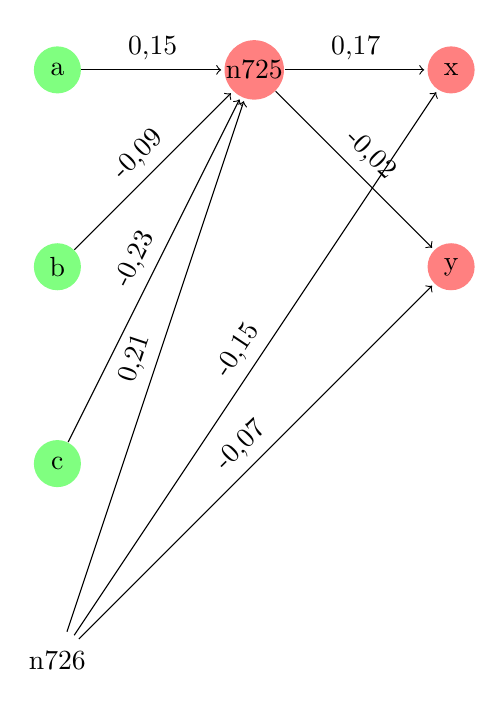
\begin{tikzpicture}[shorten >=1pt,->,draw=black!,node distance=2.5cm]
\tikzstyle{neuron}=[circle,fill=black!25,minimum size=17pt,inner sep=0pt]
\tikzstyle{constant}=[neuron, fill=white!50];
\tikzstyle{identity}=[neuron, fill=green!50];
\tikzstyle{sigmoid}=[neuron, fill=red!50];
\node [identity] (a) {a};
\node [identity,below of=a] (b) {b};
\node [identity,below of=b] (c) {c};
\node [constant,below of=c] (n726) {n726};
\node [sigmoid,right of=a] (n725) {n725};
\node [sigmoid,right of=n725] (x) {x};
\node [sigmoid,below of=x] (y) {y};
\path[every node/.style={sloped,anchor=south,auto=false}]
(b) edge node {-0,09} (n725)
(a) edge node {0,15} (n725)
(n726) edge node {0,21} (n725)
(n726) edge node {-0,07} (y)
(n726) edge node {-0,15} (x)
(c) edge node {-0,23} (n725)
(n725) edge node {-0,02} (y)
(n725) edge node {0,17} (x)
;\end{tikzpicture}
\end{document}